\begin{frame}[plain]
  \vfill
  \centering
  \Huge Multimodal LLMs in 2025--2026
  \vfill
\end{frame}

\begin{frame}{Open-Weight Flagships: Qwen-VL and InternVL}
  \begin{itemize}
    \item[{\color{red}\textbullet}] \textbf{Qwen2.5-VL} (Feb 2025): a dynamic-resolution ViT trained from
      scratch with window attention; absolute time encoding gives hours-long video comprehension with
      second-level event localization; grounding by bounding box or point; structured parsing of
      invoices, forms and tables.
    \item[{\color{red}\textbullet}] \textbf{Qwen3-VL} (Sep--Nov 2025): dense and MoE sizes from 2B to 235B,
      each in Instruct and reasoning-focused Thinking editions; native 256K context, expandable to 1M;
      operates PC and mobile GUIs as a visual agent; OCR in 32 languages.
    \item[{\color{red}\textbullet}] \textbf{InternVL3 / InternVL3.5} (2025): \emph{native multimodal
      pre-training}, one joint stage over text and multimodal corpora instead of retrofitting a finished
      text LLM; InternVL3.5 adds Cascade RL and a Visual Resolution Router for a $4\times$ inference
      speedup, reporting state of the art among open-source MLLMs.
  \end{itemize}
  \vspace{0.3em}
  {\scriptsize Bai et al., \href{https://arxiv.org/abs/2502.13923}{arXiv:2502.13923};
  Bai et al., \href{https://arxiv.org/abs/2511.21631}{arXiv:2511.21631};
  Zhu et al., \href{https://arxiv.org/abs/2504.10479}{arXiv:2504.10479};
  Wang et al., \href{https://arxiv.org/abs/2508.18265}{arXiv:2508.18265}.}
\end{frame}

\begin{frame}{Inside a 2025 Flagship: Qwen3-VL}
  \begin{figure}
    \centering
    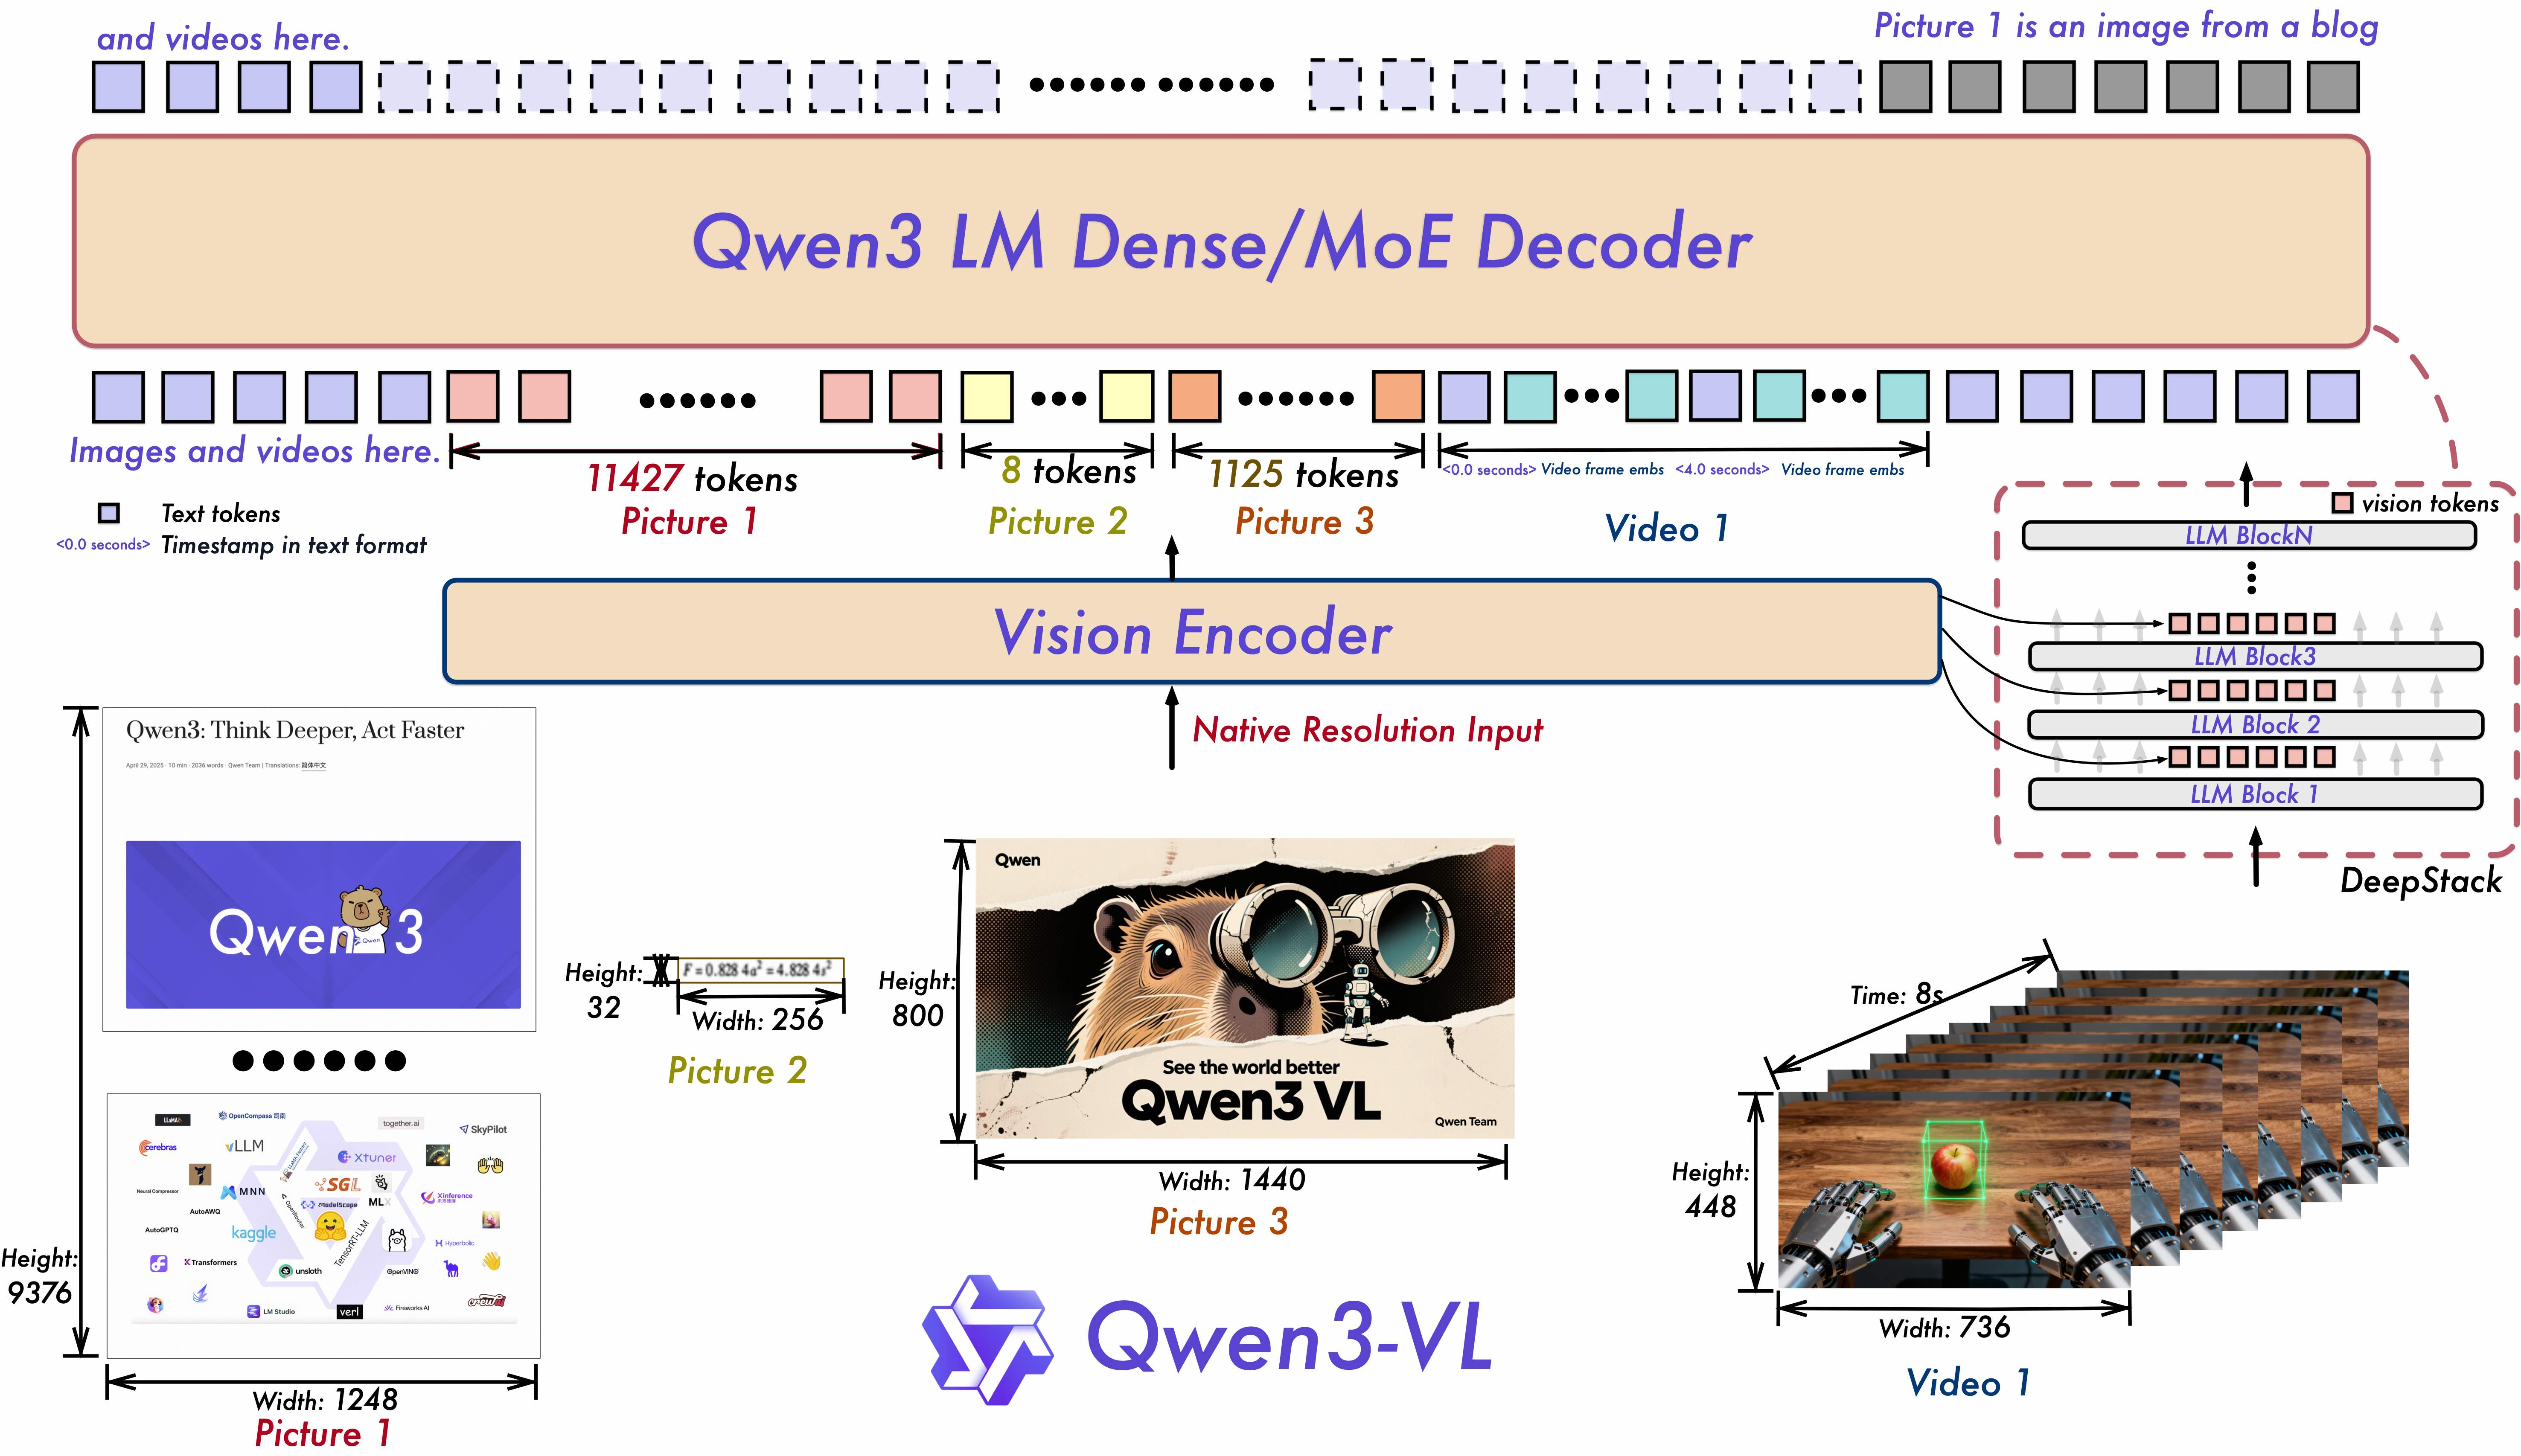
\includegraphics[width=0.94\textwidth, height=0.68\textheight, keepaspectratio]{images/multimodal-nlp/multimodal_qwen3_vl_architecture.jpg}
    \caption*{\scriptsize Native-resolution images and timestamped video frames enter one decoder as
    interleaved tokens, so token count scales with input size: 11{,}427 tokens for a long webpage, 8 for a
    small formula. DeepStack feeds multi-level ViT features into several LLM blocks. Source: Qwen team,
    Qwen3-VL repository, \href{https://arxiv.org/abs/2511.21631}{arXiv:2511.21631}.}
  \end{figure}
\end{frame}

\begin{frame}{How Modern MLLMs Are Trained}
  \begin{itemize}
    \item[{\color{red}\textbullet}] \textbf{Encoder first:} Qwen2.5-VL trains its ViT alone on 1.5T
      tokens of captions, OCR and visual knowledge while the LLM stays frozen, then trains ViT and LLM
      jointly on 2T mixed multimodal tokens.
    \item[{\color{red}\textbullet}] \textbf{Then supervised fine-tuning} on multimodal instruction data,
      exactly as for text LLMs.
    \item[{\color{red}\textbullet}] \textbf{Then reinforcement learning:} InternVL3.5's Cascade RL runs an
      offline preference stage (MPO) and then an online stage (GSPO). RL post-training algorithms are
      covered later in the course.
  \end{itemize}
  \begin{figure}
    \centering
    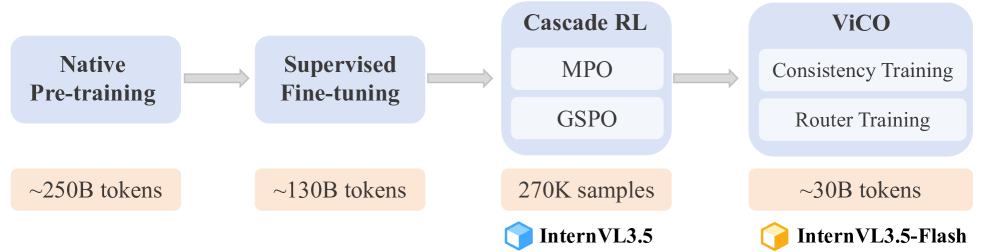
\includegraphics[width=0.76\textwidth]{images/multimodal-nlp/multimodal_internvl35_training_pipeline.png}
    \caption*{\scriptsize InternVL3.5's recipe: native pre-training, supervised fine-tuning, Cascade RL;
    the final ViCO stage trains the Flash variant's resolution router. Source: Wang et al.,
    \href{https://arxiv.org/abs/2508.18265}{arXiv:2508.18265}, Figure~3.}
  \end{figure}
\end{frame}

\begin{frame}{Frontier Systems Are Natively Multimodal}
  \begin{itemize}
    \item[{\color{red}\textbullet}] \textbf{GPT-4o} (May 2024): ``a single new model end-to-end across text,
      vision, and audio''; the same network reads and produces all of them.
    \item[{\color{red}\textbullet}] \textbf{Gemini 2.5 Pro} (Mar 2025): text, audio, images, video and whole
      code repositories in a 1M-token context window.
    \item[{\color{red}\textbullet}] \textbf{GPT-5} (Aug 2025): one unified system that decides when to think
      longer; 84.2\% on MMMU at launch.
    \item[{\color{red}\textbullet}] \textbf{Gemini 3} (Nov 2025): launched as ``the best model in the world
      for multimodal understanding'': 81\% on MMMU-Pro, 87.6\% on Video-MMMU.
    \item[{\color{red}\textbullet}] \textbf{2026 so far:} new releases land every few months (GPT-5.4 through
      5.6, Gemini 3.5 and 3.6, Claude Opus 4.7 and Fable 5); the best frontier MMMU-Pro score moved from
      81\% to 83\% without tools (84.6\% with tools) in eight months.
  \end{itemize}
  \vspace{0.3em}
  {\scriptsize Sources: OpenAI, Google and Anthropic release announcements, 2024--2026 (see references).}
\end{frame}

\begin{frame}{Thinking With Images}
  \begin{itemize}
    \item[{\color{red}\textbullet}] \textbf{OpenAI o3 and o4-mini} (Apr 2025) were the first OpenAI models
      that ``think with images in their chain-of-thought'' rather than merely looking at them.
    \item[{\color{red}\textbullet}] During reasoning the model crops, zooms into and rotates the user's
      image, natively and without separate specialist models, and can mix these steps with web search
      and Python.
    \item[{\color{red}\textbullet}] Result: state of the art at the time on MMMU, MathVista and chart
      reasoning, and 95.7\% on the V* visual-search benchmark, ``largely solving'' it.
    \item[{\color{red}\textbullet}] The pattern generalizes: perception becomes a sequence of
      \emph{actions} on the input, interleaved with textual reasoning. How such reasoning is trained is
      covered later in the course.
  \end{itemize}
  \vspace{0.4em}
  {\scriptsize OpenAI, ``Thinking with images'', April 2025,
  \href{https://openai.com/index/thinking-with-images/}{openai.com/index/thinking-with-images}.}
\end{frame}

\begin{frame}{Native Multimodality: Early Fusion Returns}
  \begin{itemize}
    \item[{\color{red}\textbullet}] The projector recipe bolts vision onto a finished LLM. The native
      alternative pretrains one transformer on every modality tokenized together: \textbf{Chameleon}
      (Meta, 2024) maps a 512$\times$512 image to 1024 discrete tokens, and one autoregressive model
      reads and writes both modalities.
    \item[{\color{red}\textbullet}] \textbf{Llama 4} (Apr 2025): Meta's first open-weight family pretrained
      with early fusion, jointly on text, image and video data.
    \item[{\color{red}\textbullet}] Across 457 trained models, late fusion showed no inherent advantage;
      early fusion is stronger at small scales and cheaper to train (Shukor et al., ICCV 2025).
  \end{itemize}
  \begin{figure}
    \centering
    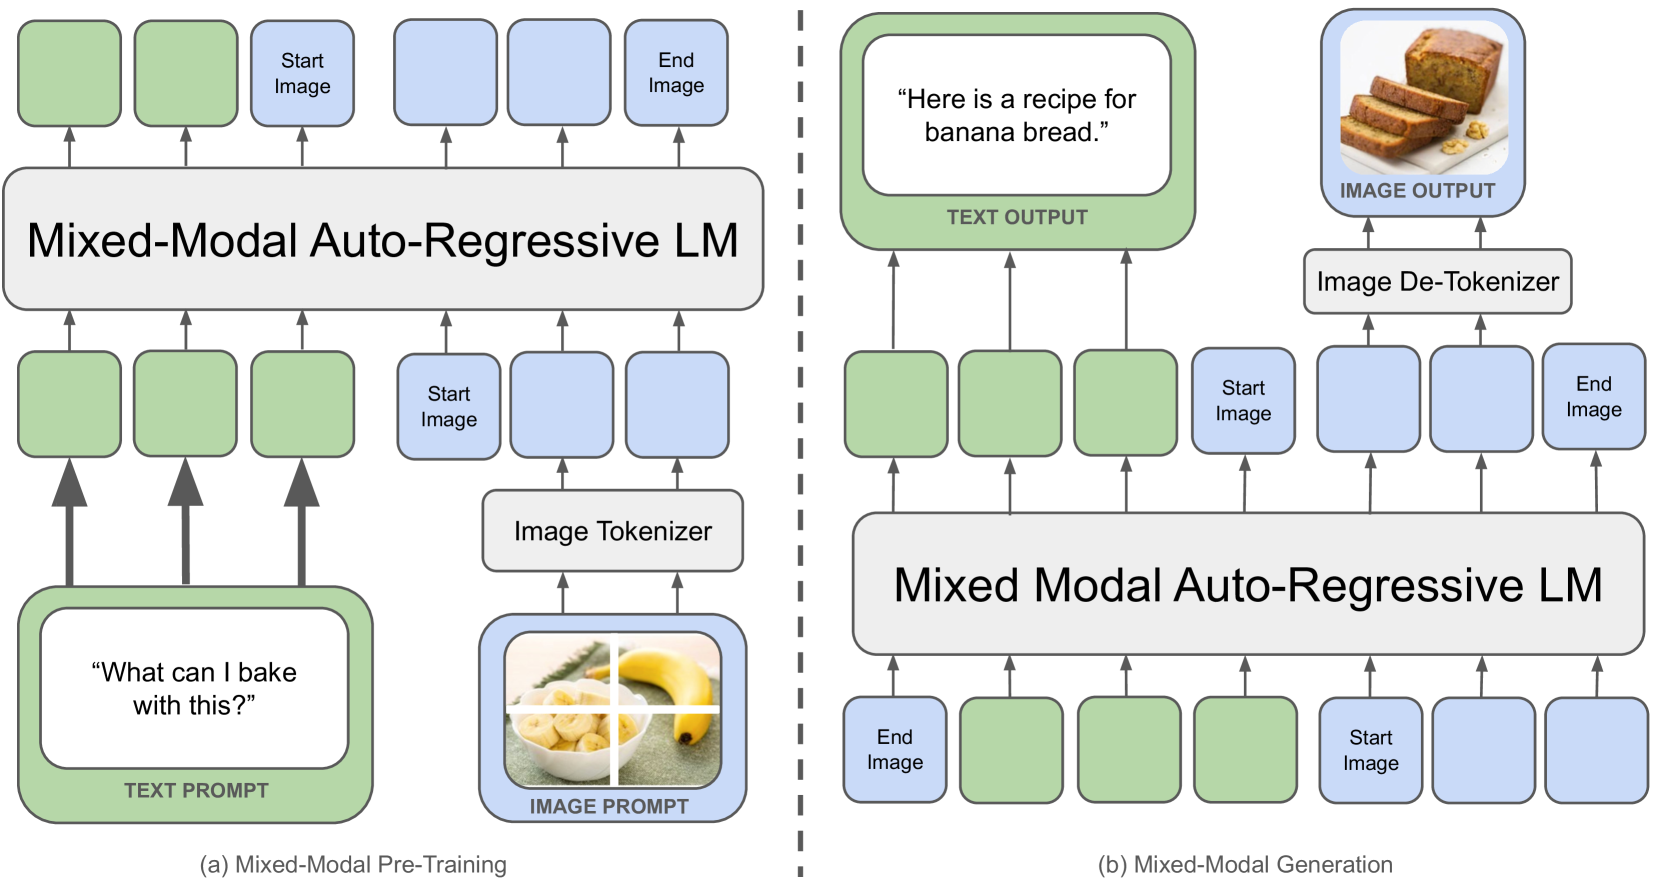
\includegraphics[width=0.66\textwidth, height=0.31\textheight, keepaspectratio]{images/multimodal-nlp/multimodal_chameleon_mixed_modal_tokens.png}
    \caption*{\scriptsize Source: Chameleon Team, \href{https://arxiv.org/abs/2405.09818}{arXiv:2405.09818}, Figure~1.}
  \end{figure}
\end{frame}

\begin{frame}{Unified Models: Understanding and Generation}
  \begin{itemize}
    \item[{\color{red}\textbullet}] \textbf{Transfusion} (ICLR 2025): one transformer, two losses:
      next-token prediction on text tokens, a diffusion objective on continuous image patches in the
      same sequence; scales better than quantizing images.
    \item[{\color{red}\textbullet}] \textbf{Janus-Pro} (DeepSeek, Jan 2025): decoupled visual encoding:
      SigLIP features for understanding, VQ tokens for generation, one shared autoregressive core.
    \item[{\color{red}\textbullet}] \textbf{In production:} GPT-4o image generation (Mar 2025) and Gemini
      2.5 Flash Image (``Nano Banana'', Aug 2025) put native image generation and editing in assistants;
      Nano Banana Pro (Nov 2025) grounds generations in live search.
  \end{itemize}
  \begin{figure}
    \centering
    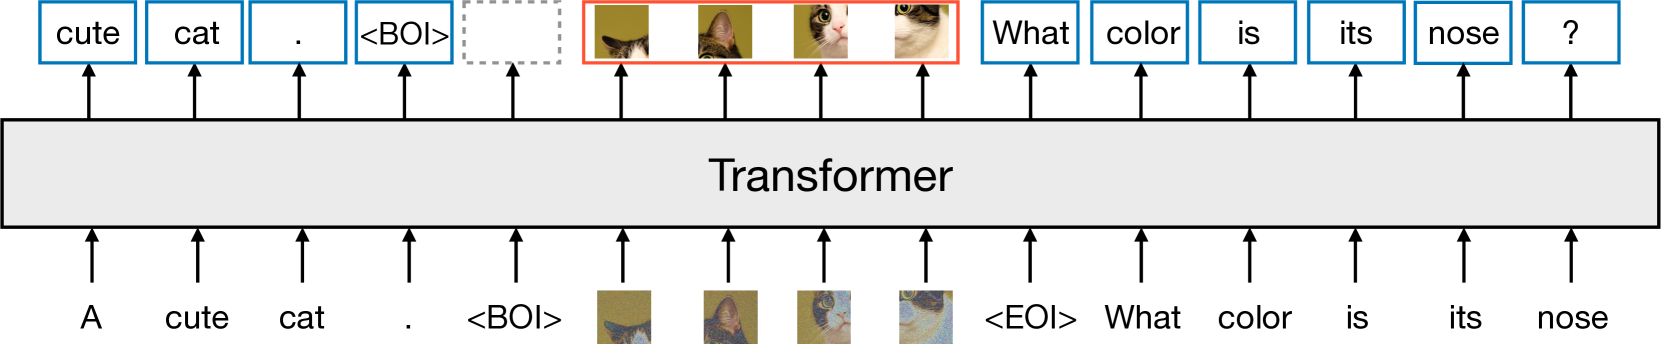
\includegraphics[width=0.72\textwidth]{images/multimodal-nlp/multimodal_transfusion_text_diffusion_one_transformer.png}
    \caption*{\scriptsize One sequence mixes text tokens with continuous image patches between
    \texttt{<BOI>}/\texttt{<EOI>}. Source: Zhou et al., ICLR 2025,
    \href{https://arxiv.org/abs/2408.11039}{arXiv:2408.11039}, Figure~1.}
  \end{figure}
\end{frame}

\begin{frame}{Omni Models: Speech In, Speech Out}
  \begin{columns}[T,onlytextwidth]
    \column{0.55\textwidth}
      \begin{itemize}
        \item[{\color{red}\textbullet}] \textbf{GPT-4o} answers speech in 320\,ms on average; the cascaded
          pipeline it replaced (transcription, text LLM, TTS) took 2.8--5.4\,s and lost tone, multiple
          speakers and laughter.
        \item[{\color{red}\textbullet}] \textbf{Qwen2.5-Omni} (Mar 2025): \textbf{Thinker-Talker}: the
          Thinker LLM writes text while the Talker streams speech tokens from its hidden states; TMRoPE
          keeps audio and video frames on one timeline.
        \item[{\color{red}\textbullet}] \textbf{Qwen3-Omni} (Sep 2025): both parts become MoE; 234\,ms
          theoretical first-packet latency; open-source state of the art on 32 of 36 audio and
          audio-visual benchmarks. \textbf{Qwen3.5-Omni} (Apr 2026) scales to a 256K context and over
          ten hours of audio input.
        \item[{\color{red}\textbullet}] Speech and audio processing get their own treatment later in the
          course.
      \end{itemize}
    \column{0.42\textwidth}
      \begin{figure}
        \centering
        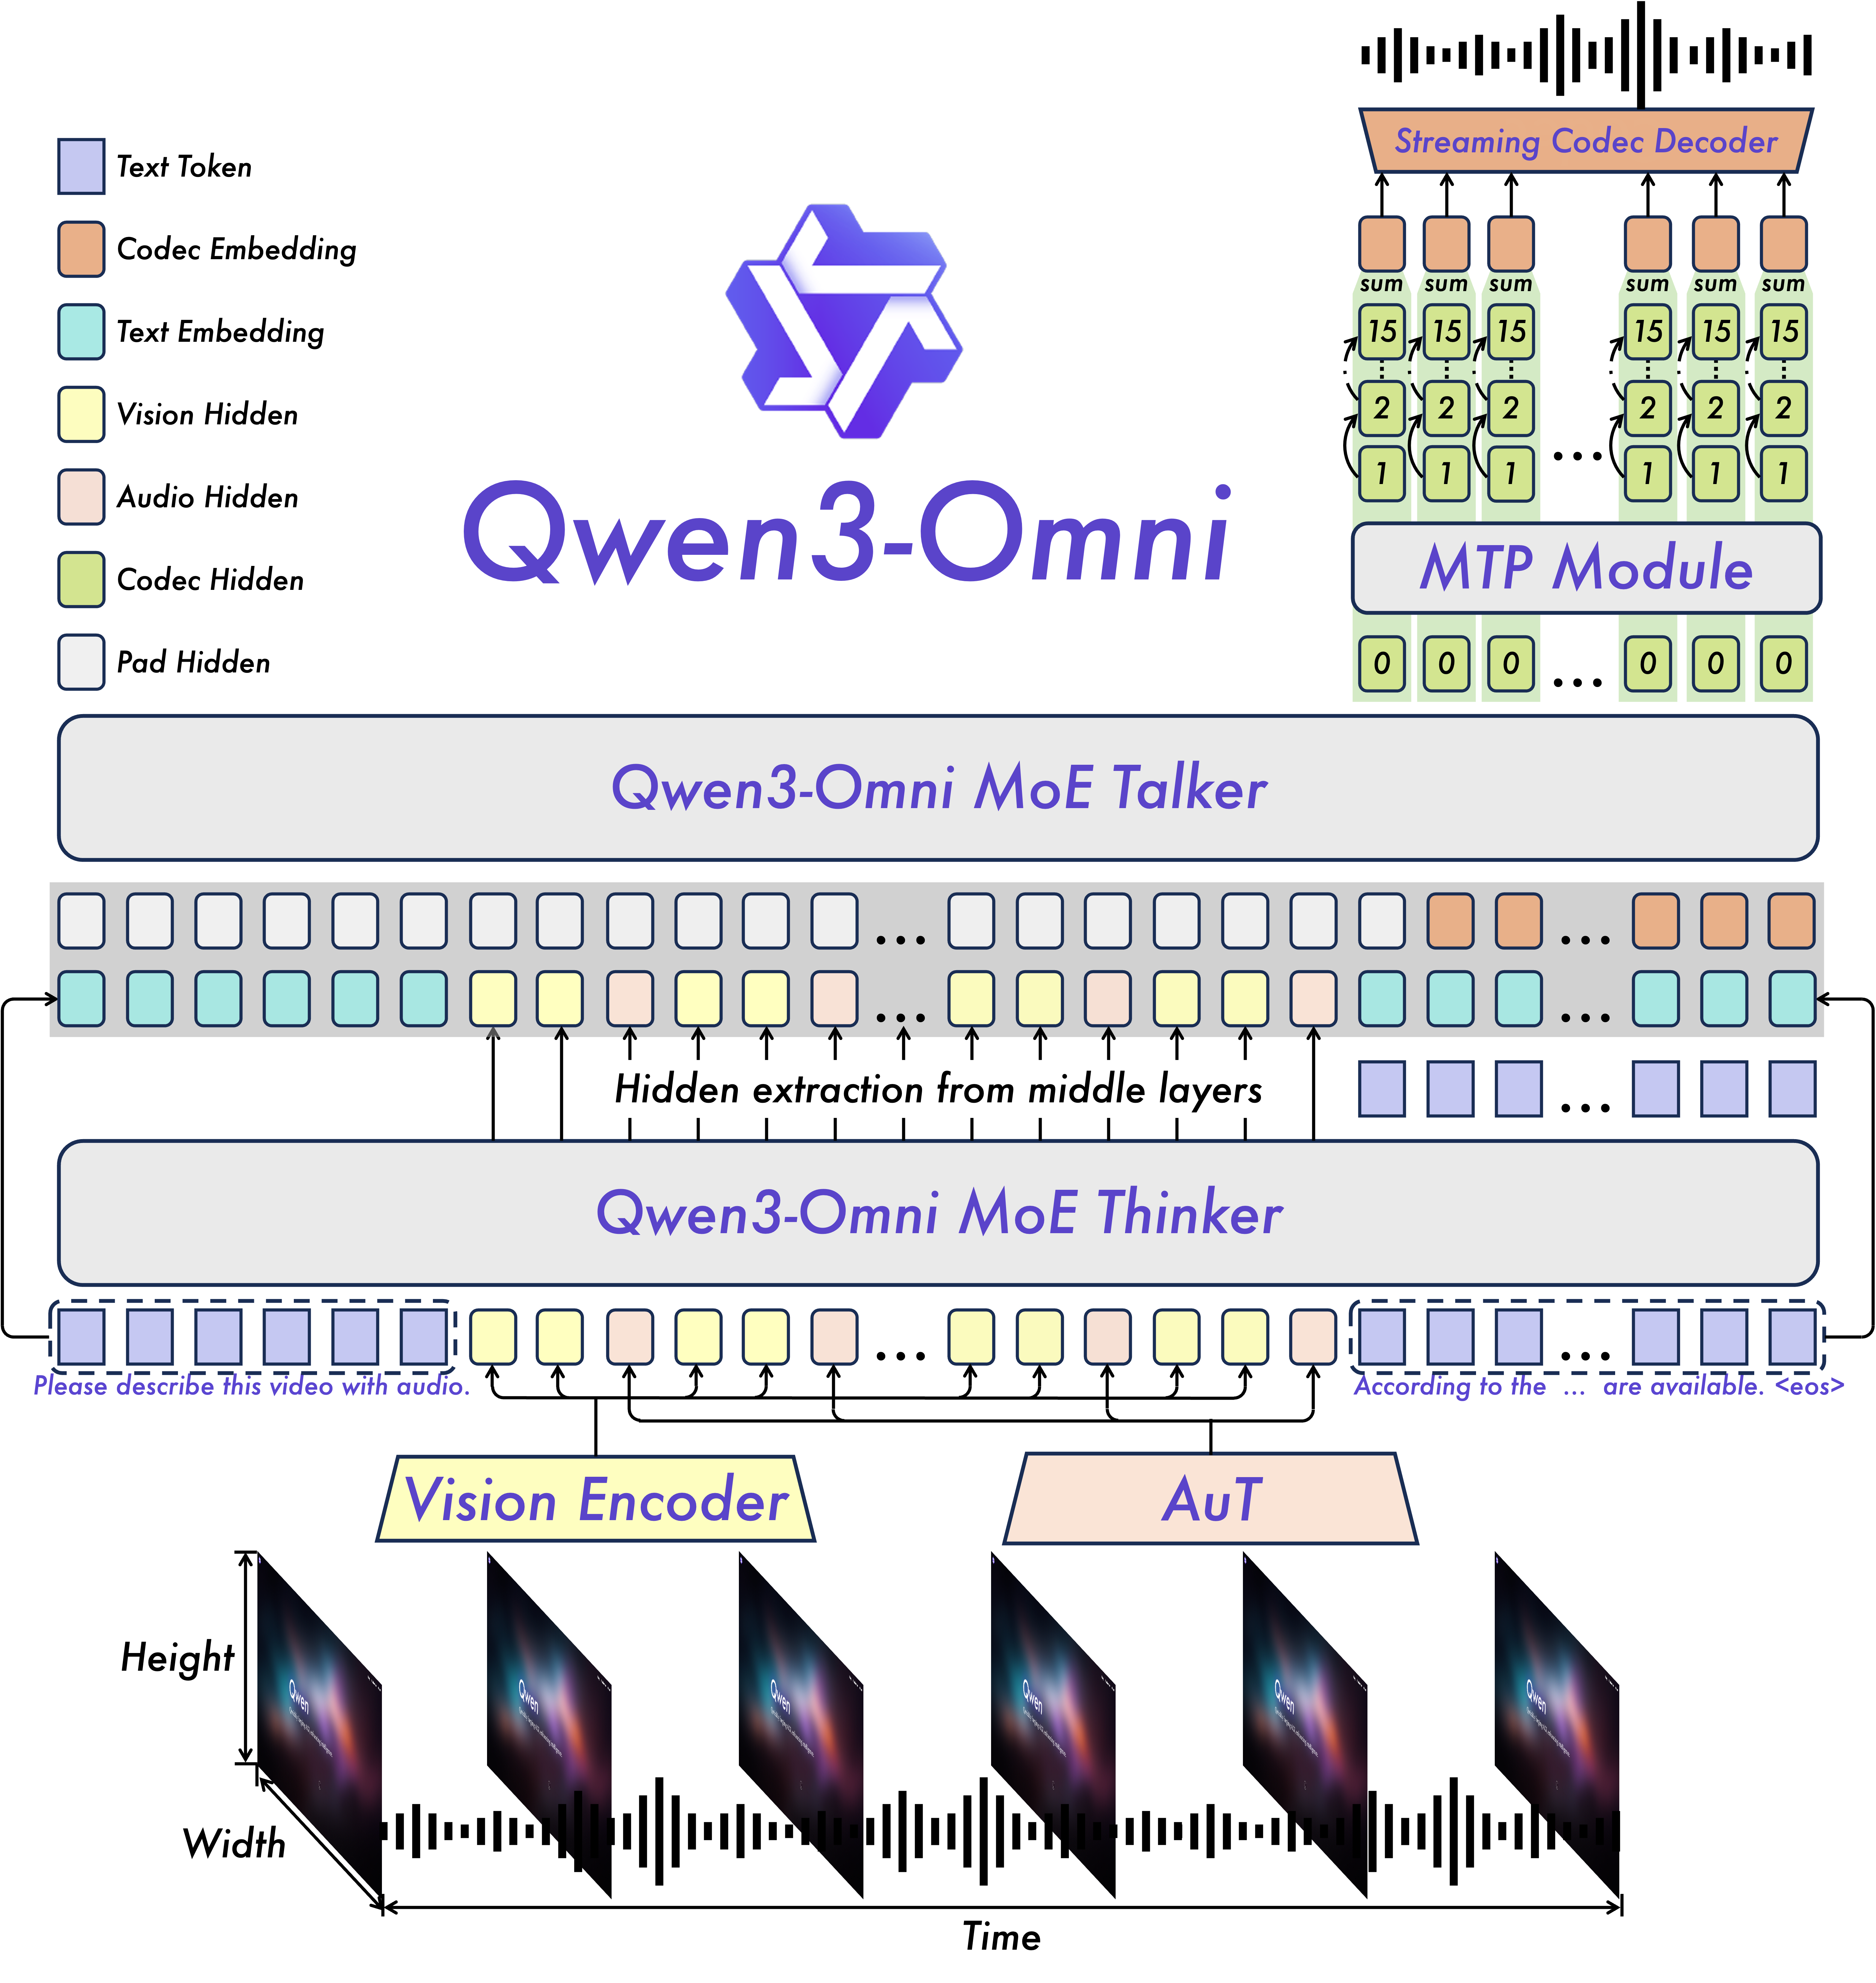
\includegraphics[width=\linewidth, height=0.7\textheight, keepaspectratio]{images/multimodal-nlp/multimodal_qwen3_omni_thinker_talker.png}
        \caption*{\scriptsize Source: Xu et al., ``Qwen3-Omni Technical Report'',
        \href{https://arxiv.org/abs/2509.17765}{arXiv:2509.17765}, Figure~2.}
      \end{figure}
  \end{columns}
\end{frame}

\begin{frame}{Video Understanding}
  \begin{itemize}
    \item[{\color{red}\textbullet}] Video enters the model as resized frames plus timestamps. Gemini
      spends roughly 300 tokens per second of video, so a 1M-token context holds about an hour.
    \item[{\color{red}\textbullet}] Qwen2.5-VL's absolute time encoding localizes events to the second
      inside hours-long video.
    \item[{\color{red}\textbullet}] \textbf{Video-MME} (CVPR 2025): 900 videos totalling 254 hours with
      2{,}700 expert QA pairs, durations from 11 seconds to an hour. Gemini 1.5 Pro led at release with
      75\% (no subtitles), and every model degrades as the video gets longer.
  \end{itemize}
  \begin{figure}
    \centering
    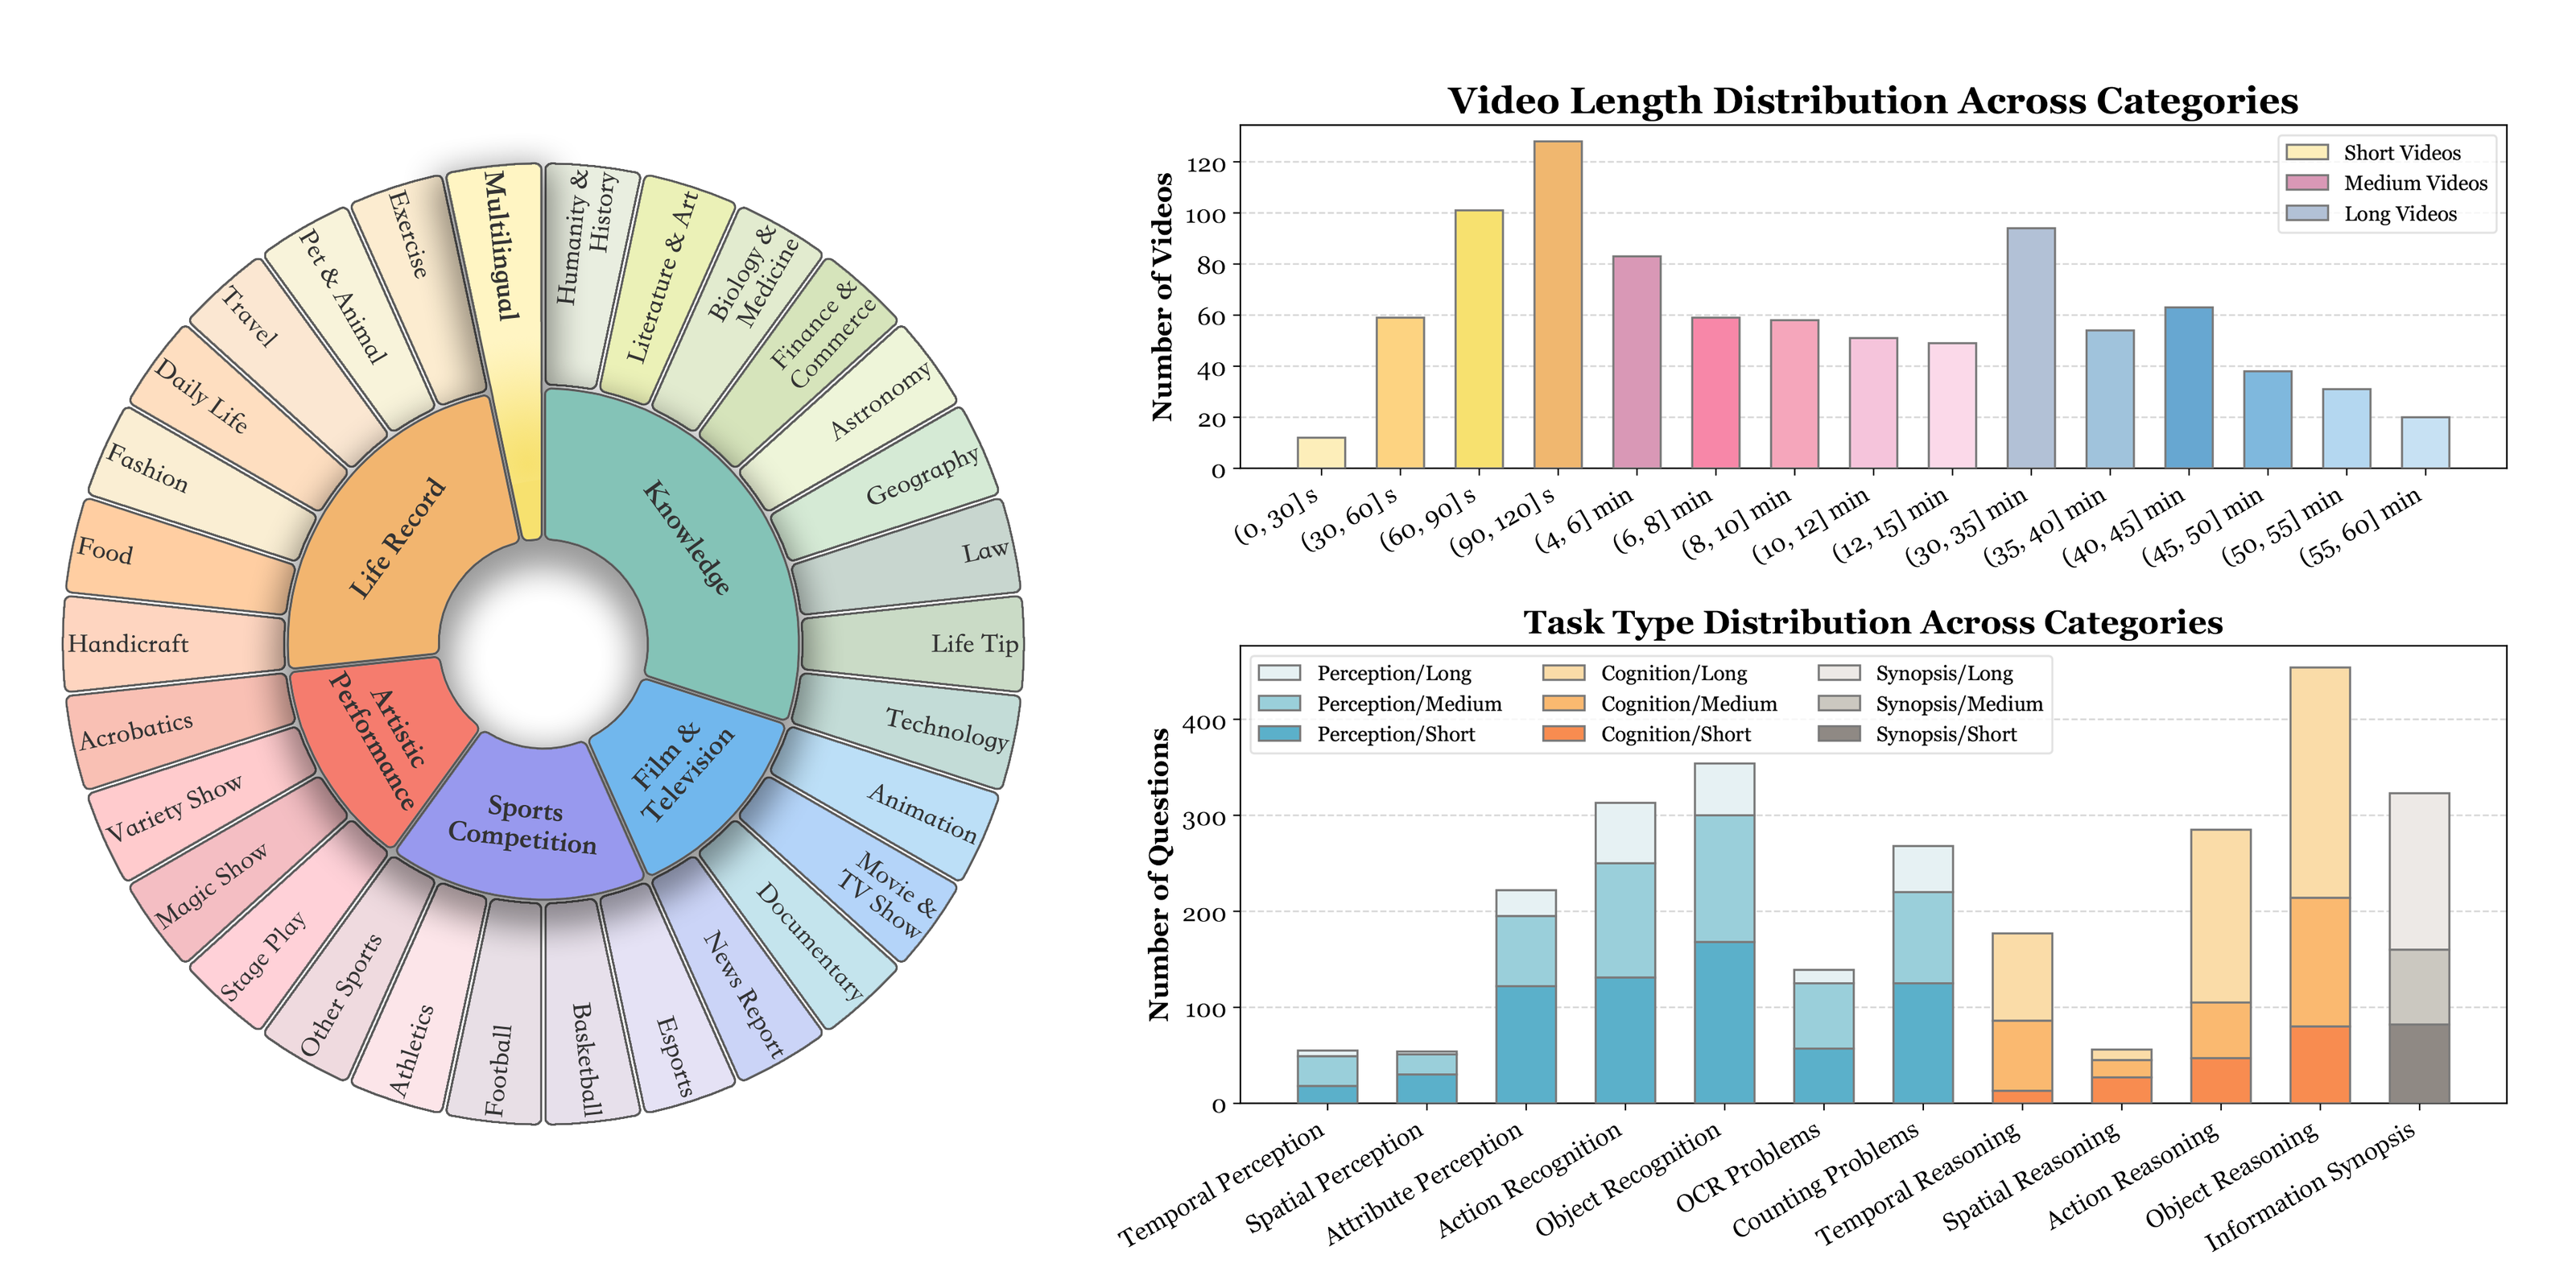
\includegraphics[width=0.68\textwidth, height=0.36\textheight, keepaspectratio]{images/multimodal-nlp/multimodal_video_mme_benchmark_composition.png}
    \caption*{\scriptsize Source: Fu et al., ``Video-MME'', CVPR 2025,
    \href{https://arxiv.org/abs/2405.21075}{arXiv:2405.21075}, Figure~2.}
  \end{figure}
\end{frame}

\begin{frame}{Documents: The Everyday Workload}
  \begin{itemize}
    \item[{\color{red}\textbullet}] Invoices, forms, tables, charts and scanned pages are where most users
      meet these models. DocVQA and ChartQA (covered earlier) defined the tasks; document parsing is now
      a headline capability of every flagship.
    \item[{\color{red}\textbullet}] \textbf{Qwen2.5-VL} turns document pages into structured output and
      analyzes charts, diagrams and layouts.
    \item[{\color{red}\textbullet}] \textbf{OmniDocBench} (CVPR 2025) evaluates end-to-end document
      parsing across nine source types, from academic papers and textbooks to handwriting and densely
      typeset newspapers.
    \item[{\color{red}\textbullet}] Frontier labs report against it: OpenAI cites GPT-5.4 cutting its
      OmniDocBench error to 0.109 from GPT-5.2's 0.140.
  \end{itemize}
  \vspace{0.3em}
  {\scriptsize Ouyang et al., \href{https://arxiv.org/abs/2412.07626}{arXiv:2412.07626};
  OpenAI, ``Introducing GPT-5.4'', March 2026,
  \href{https://openai.com/index/introducing-gpt-5-4/}{openai.com/index/introducing-gpt-5-4}.}
\end{frame}

\begin{frame}{Retrieval Without OCR: ColPali}
  \begin{itemize}
    \item[{\color{red}\textbullet}] Retrieval-augmented generation (covered earlier) assumes clean text.
      Real corpora arrive as page images whose figures, tables and layout an OCR pipeline flattens or
      loses.
    \item[{\color{red}\textbullet}] \textbf{ColPali} (ICLR 2025) embeds the page image directly: a
      vision-language model produces multi-vector embeddings, matched to the query with ColBERT-style
      late interaction.
    \item[{\color{red}\textbullet}] It outperforms the OCR pipelines while indexing pages an order of
      magnitude faster: 0.39\,s against 7.22\,s per page in the paper's comparison.
  \end{itemize}
  \begin{figure}
    \centering
    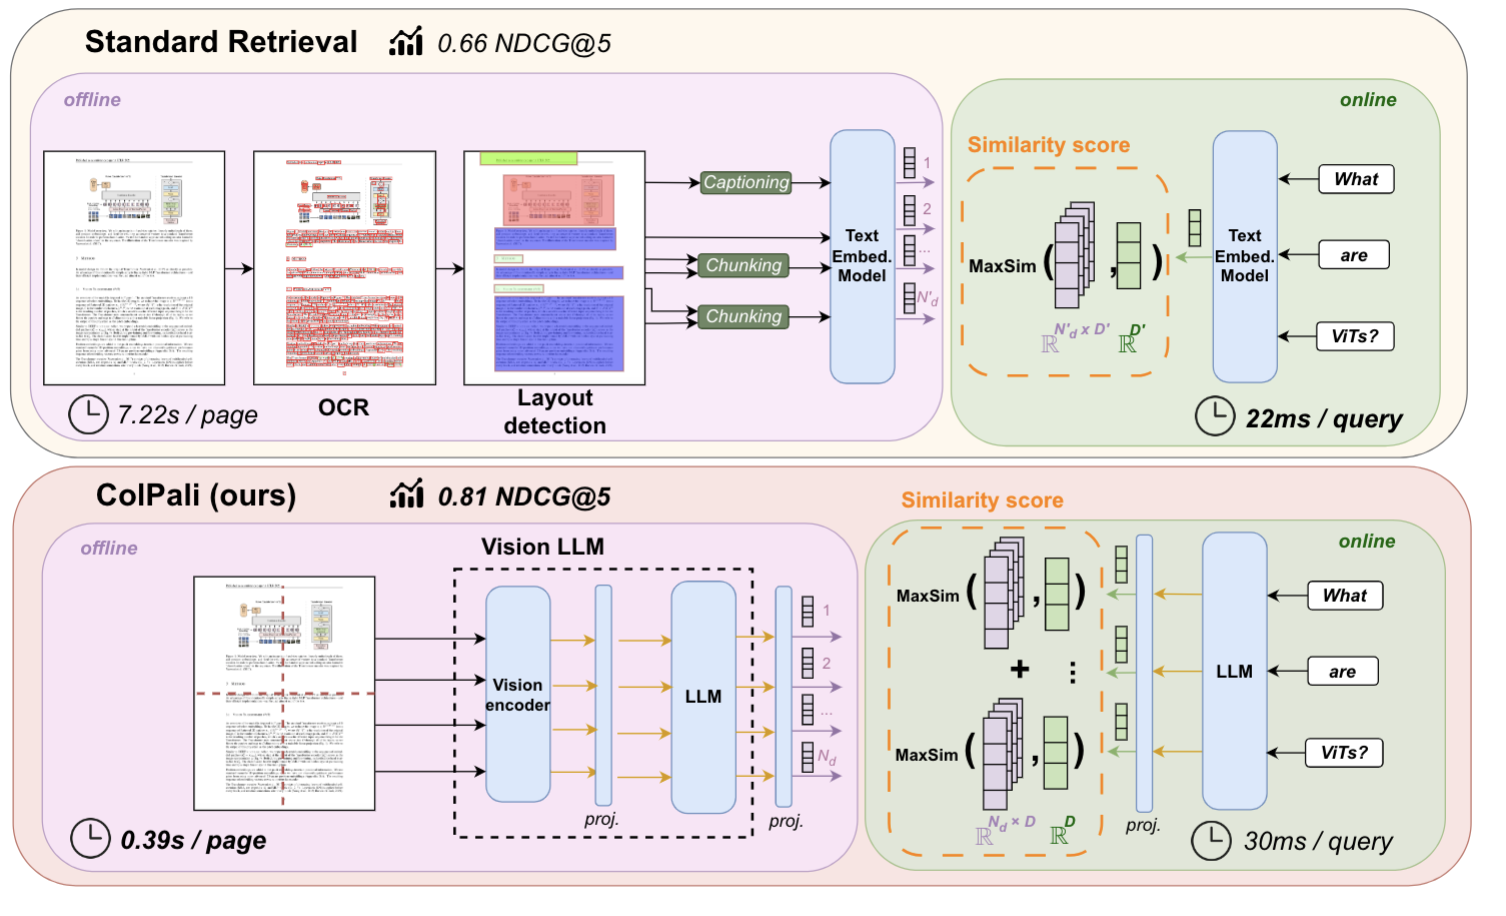
\includegraphics[width=0.6\textwidth, height=0.44\textheight, keepaspectratio]{images/multimodal-nlp/multimodal_colpali_late_interaction_retrieval.png}
    \caption*{\scriptsize Source: Faysse et al., ``ColPali'', ICLR 2025,
    \href{https://arxiv.org/abs/2407.01449}{arXiv:2407.01449}, Figure~1.}
  \end{figure}
\end{frame}

\begin{frame}{GUI Grounding and Computer Use}
  \begin{itemize}
    \item[{\color{red}\textbullet}] \textbf{The perception task:} map an instruction to the right pixel.
      ScreenSpot (ACL 2024) tests grounding on 600+ screenshots across mobile, desktop and web;
      ScreenSpot-Pro moves to high-resolution professional software, where the best grounding model at
      its release managed 18.9\%.
    \item[{\color{red}\textbullet}] \textbf{The benchmark:} OSWorld (NeurIPS 2024): 369 real tasks in
      real operating systems, scored by executing the resulting state.
    \item[{\color{red}\textbullet}] \textbf{The products:} Claude computer use (Oct 2024, the first
      frontier model to offer it), OpenAI Operator (Jan 2025) and Gemini 2.5 Computer Use (Oct 2025) all
      run the same loop: screenshot in, click or keystroke out.
    \item[{\color{red}\textbullet}] \textbf{The trajectory:} Anthropic reports its models moving from
      under 15\% on OSWorld in late 2024 to 72.5\% by early 2026. The agent architectures around this
      loop are covered later in the course.
  \end{itemize}
  \vspace{0.3em}
  {\scriptsize Cheng et al., \href{https://arxiv.org/abs/2401.10935}{arXiv:2401.10935};
  Li et al., \href{https://arxiv.org/abs/2504.07981}{arXiv:2504.07981};
  Xie et al., \href{https://arxiv.org/abs/2404.07972}{arXiv:2404.07972};
  Anthropic, Feb 2026, \href{https://www.anthropic.com/news/acquires-vercept}{anthropic.com/news/acquires-vercept}.}
\end{frame}

\begin{frame}{Vision-Language-Action: From Screens to Robots}
  \begin{columns}[T,onlytextwidth]
    \column{0.5\textwidth}
      \begin{itemize}
        \item[{\color{red}\textbullet}] \textbf{RT-2} (CoRL 2023): fine-tune a VLM on robot trajectories
          with actions written as text tokens; web-scale knowledge transfers to manipulation.
        \item[{\color{red}\textbullet}] \textbf{OpenVLA} (CoRL 2024): open 7B model trained on 970k
          demonstrations; fused DINOv2 and SigLIP features into a Llama 2 backbone, 7-D actions out.
        \item[{\color{red}\textbullet}] \textbf{$\pi_0$} (2024): a 300M flow-matching action expert on a
          PaliGemma VLM emits continuous action chunks; $\pi_{0.5}$ (2025) generalizes to unseen homes.
        \item[{\color{red}\textbullet}] \textbf{Gemini Robotics} (2025): Gemini 2.0 as a VLA; the 1.5
          release pairs an embodied-reasoning VLM with a separate acting VLA it instructs.
      \end{itemize}
    \column{0.46\textwidth}
      \begin{figure}
        \centering
        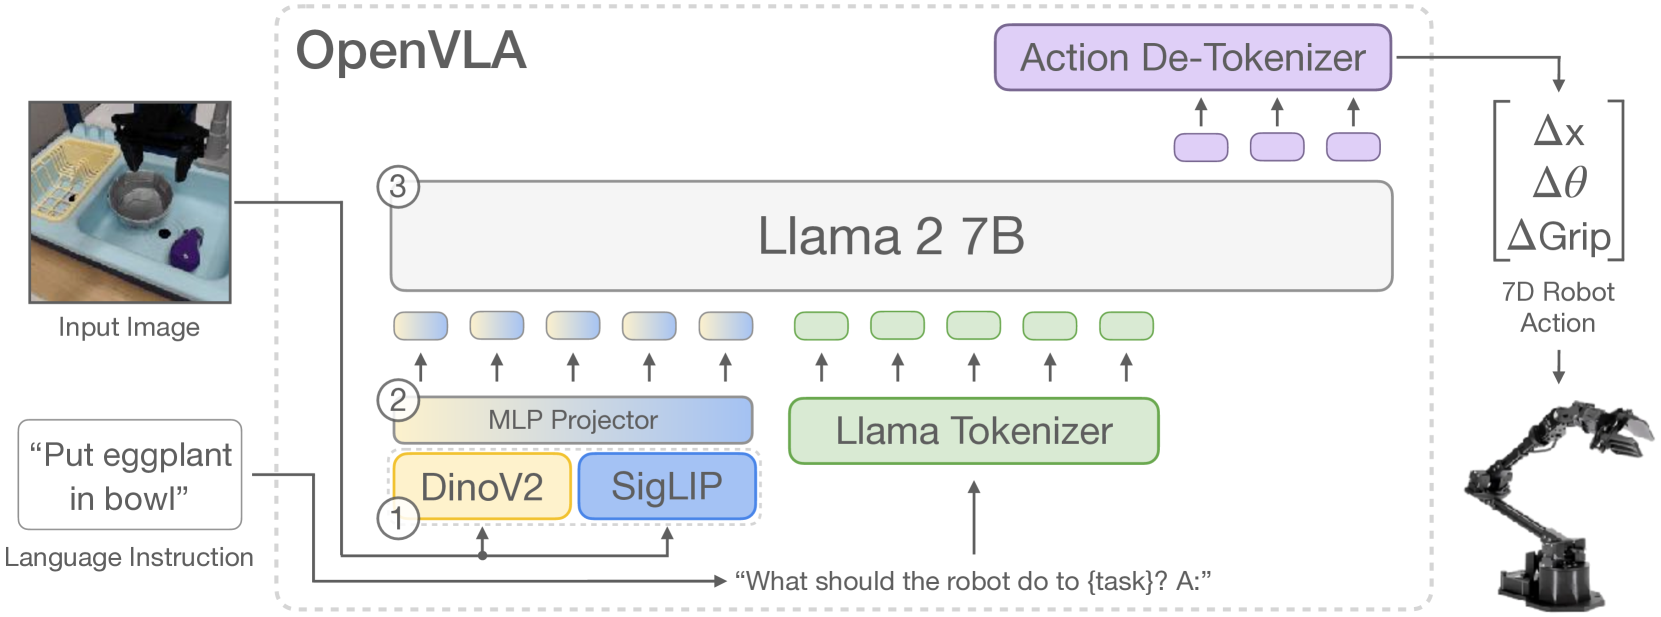
\includegraphics[width=\linewidth, height=0.62\textheight, keepaspectratio]{images/multimodal-nlp/multimodal_openvla_architecture.png}
        \caption*{\scriptsize Source: Kim et al., ``OpenVLA'', CoRL 2024,
        \href{https://arxiv.org/abs/2406.09246}{arXiv:2406.09246}, Figure~1.}
      \end{figure}
  \end{columns}
\end{frame}

\begin{frame}{Small Models: Multimodal On-Device}
  \begin{itemize}
    \item[{\color{red}\textbullet}] \textbf{SmolVLM} (2025): 256M, 500M and 2.2B models; the smallest
      runs in under 1\,GB of GPU memory.
    \item[{\color{red}\textbullet}] \textbf{PaliGemma 2} (2024) and \textbf{Gemma 3} (2025): SigLIP
      encoders on Gemma LLMs; Gemma 3's 4B, 12B and 27B models share one frozen 417M-parameter encoder.
    \item[{\color{red}\textbullet}] \textbf{Most visual tokens are wasted anyway:} FastV (ECCV 2024)
      prunes half of them after layer 2, training-free, cutting FLOPs by 45\% with negligible loss.
  \end{itemize}
  \begin{figure}
    \centering
    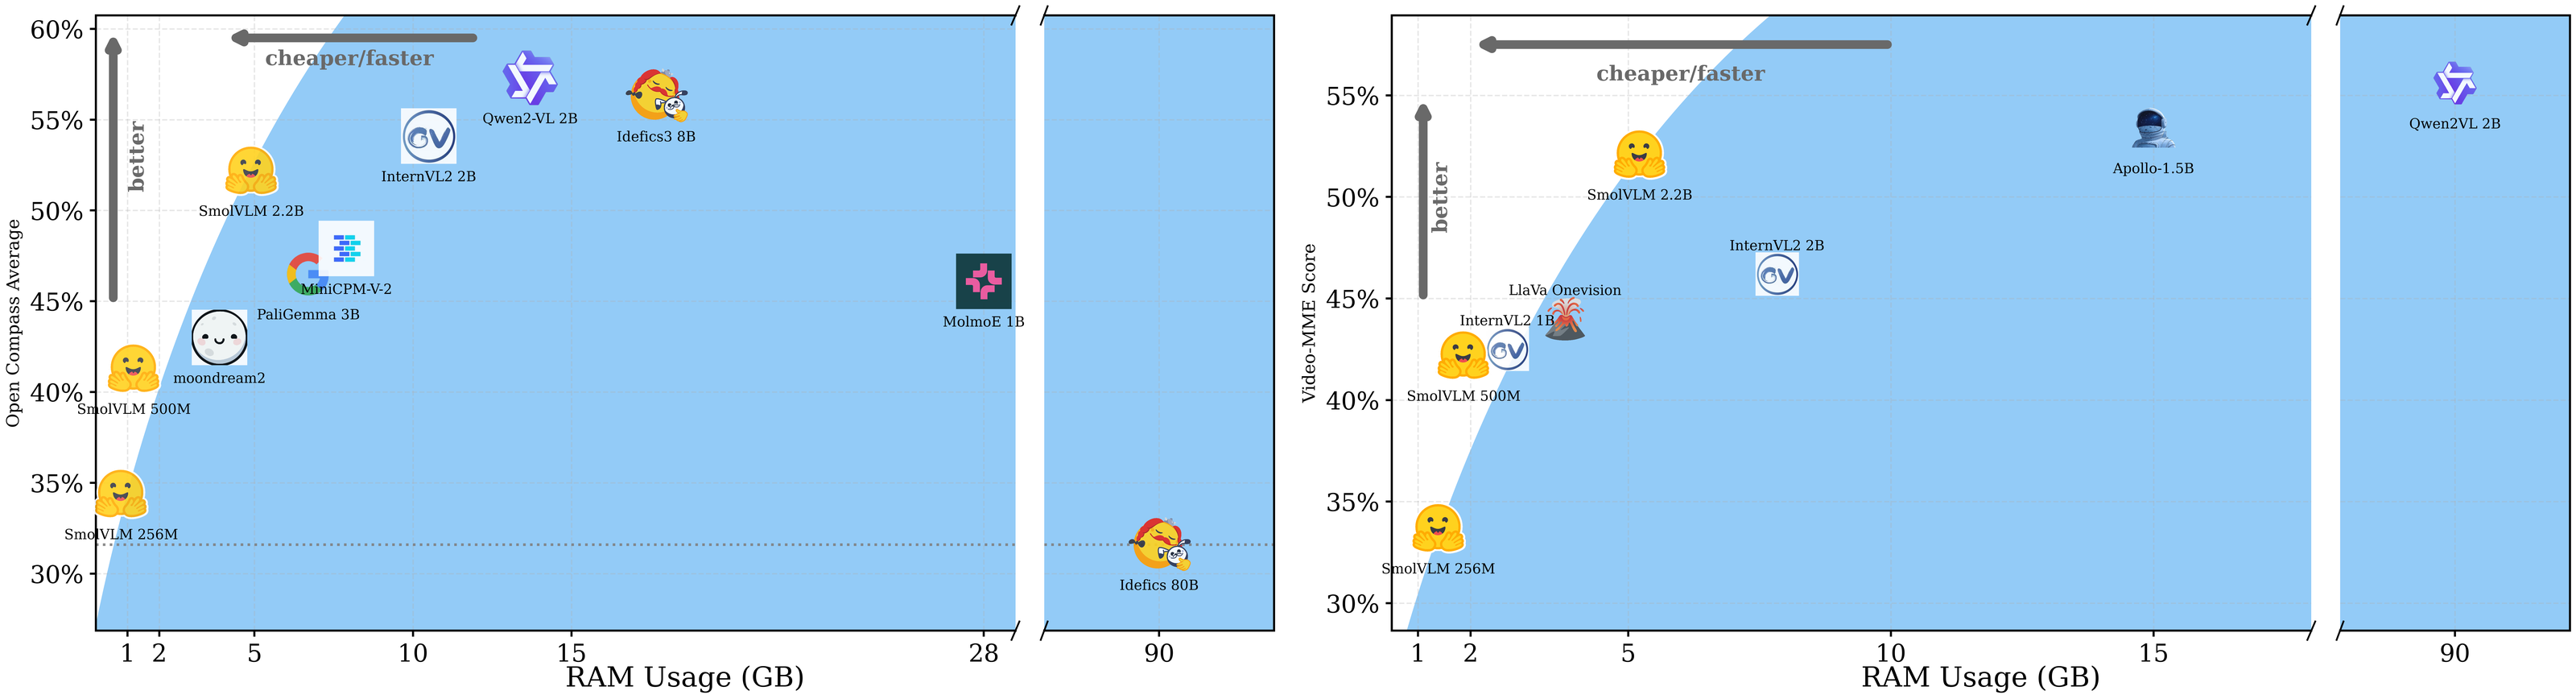
\includegraphics[width=0.82\textwidth]{images/multimodal-nlp/multimodal_smolvlm_performance_vs_memory.png}
    \caption*{\scriptsize Benchmark average against GPU memory. Source: Marafioti et al., ``SmolVLM'',
    \href{https://arxiv.org/abs/2504.05299}{arXiv:2504.05299}, Figure~1.}
  \end{figure}
\end{frame}

\begin{frame}{Evaluating Multimodal LLMs}
  \begin{columns}[T,onlytextwidth]
    \column{0.5\textwidth}
      \begin{itemize}
        \item[{\color{red}\textbullet}] \textbf{MMMU} (CVPR 2024): 11.5K college-level questions across six
          disciplines, 30 subjects and 30 image types, from charts and maps to music sheets and chemical
          structures. GPT-4V managed 56\% at launch; the strongest human-expert baseline is 88.6\%.
        \item[{\color{red}\textbullet}] \textbf{MMMU-Pro} (ACL 2025) filters out questions text-only models
          can answer, widens choices to ten, and adds a vision-only setting where the question itself is
          an image. Scores drop by 16.8 to 26.9 points.
        \item[{\color{red}\textbullet}] By mid-2026 the best systems reach the mid-80s on MMMU and the
          low-80s on MMMU-Pro, brushing the estimated 85.4\% human-expert baseline there.
      \end{itemize}
    \column{0.46\textwidth}
      \begin{figure}
        \centering
        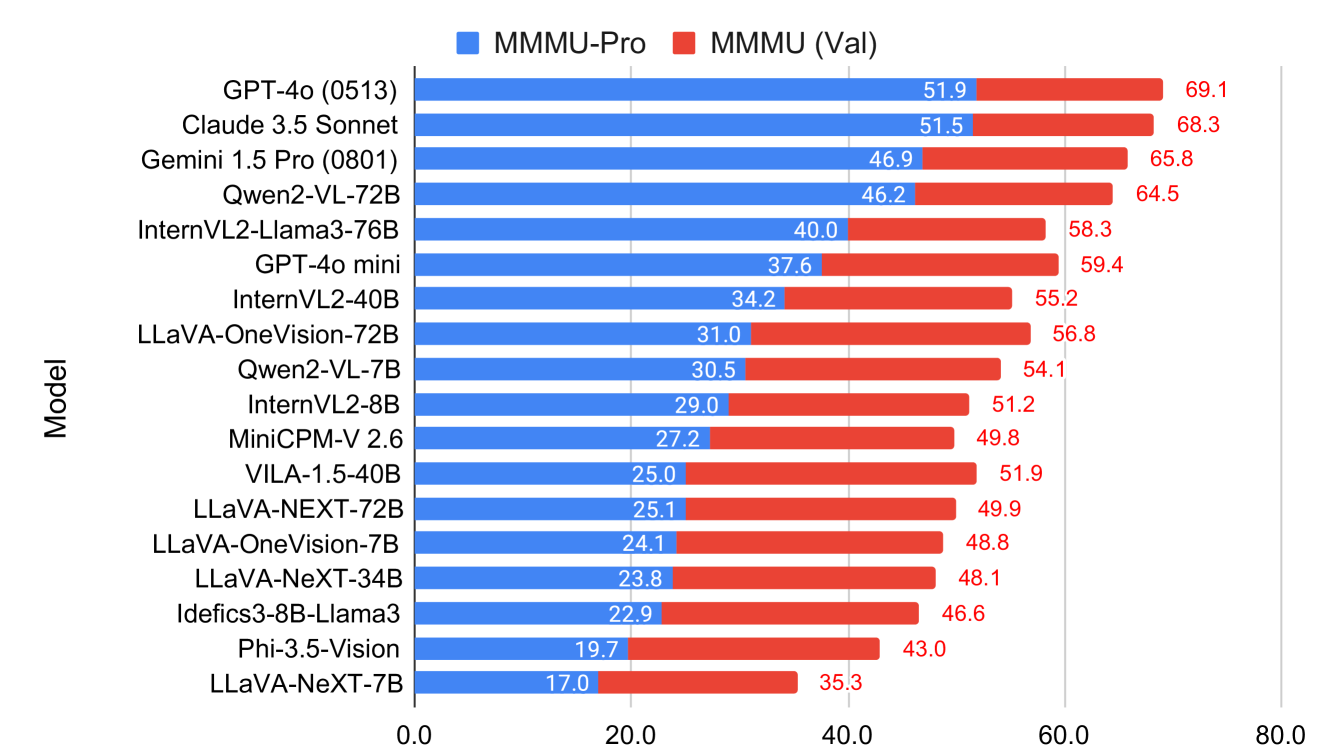
\includegraphics[width=\linewidth, height=0.66\textheight, keepaspectratio]{images/multimodal-nlp/multimodal_mmmu_pro_vs_mmmu_scores.png}
        \caption*{\scriptsize The same models on both benchmarks: every model loses ground on MMMU-Pro.
        Source: Yue et al., ``MMMU-Pro'', ACL 2025, \href{https://arxiv.org/abs/2409.02813}{arXiv:2409.02813}
        (v1), Figure~1.}
      \end{figure}
  \end{columns}
\end{frame}

\begin{frame}{What Still Fails}
  \begin{itemize}
    \item[{\color{red}\textbullet}] \textbf{Object hallucination.} Multimodal LLMs describe objects that are
      not in the image, especially objects that are frequent in, or co-occur with, what they saw in
      training. POPE (EMNLP 2023) measures this with polling-style yes/no probes.
    \item[{\color{red}\textbullet}] \textbf{Visual tokens are expensive.} A long webpage screenshot costs
      11{,}427 tokens in Qwen3-VL's own example. DeepSeek-OCR (Oct 2025) inverts the problem, rendering
      text as an image and reading it back: at a compression ratio below $10\times$ it decodes with
      97\% precision (``contexts optical compression'').
    \item[{\color{red}\textbullet}] \textbf{Evaluation is fragile.} Benchmark questions leak into training
      data, and multiple-choice scores overstate perception: MMMU-Pro's vision-only setting exists
      because models were often reading the question, not the image.
    \item[{\color{red}\textbullet}] \textbf{The attack surface grows with each modality:} instructions can
      be embedded in images and audio where text-level filters never look. Safety for agentic systems is
      covered later in the course.
  \end{itemize}
  \vspace{0.3em}
  {\scriptsize Li et al., \href{https://arxiv.org/abs/2305.10355}{arXiv:2305.10355};
  Wei et al., \href{https://arxiv.org/abs/2510.18234}{arXiv:2510.18234}.}
\end{frame}

\begin{frame}{Mitigating Hallucination}
  \begin{itemize}
    \item[{\color{red}\textbullet}] \textbf{Fix the data:} RLHF-V (CVPR 2024) collects segment-level human
      \emph{corrections} of hallucinated spans and trains on them with dense preference optimization;
      1.4k fine-grained corrections already cut object hallucination sharply.
    \item[{\color{red}\textbullet}] \textbf{Fix the decoding:} Visual Contrastive Decoding (CVPR 2024)
      needs no training at all: contrast the token distribution given the real image against the one
      given a noised copy, and the language prior's contribution cancels out.
  \end{itemize}
  \begin{figure}
    \centering
    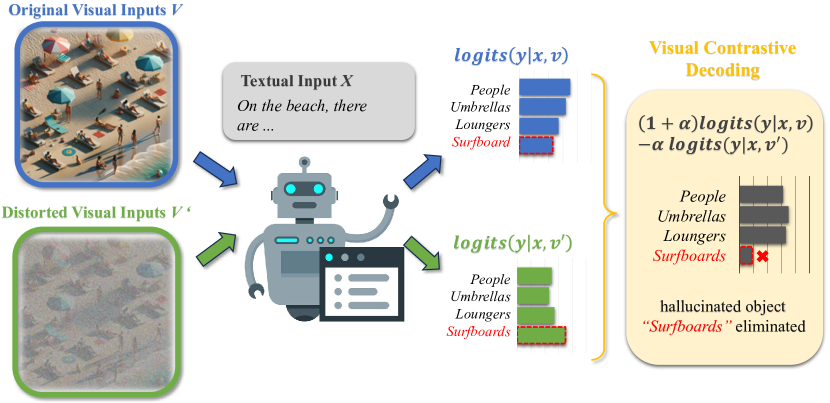
\includegraphics[width=0.62\textwidth, height=0.38\textheight, keepaspectratio]{images/multimodal-nlp/multimodal_vcd_contrastive_decoding_hallucination.png}
    \caption*{\scriptsize Source: Leng et al., ``Visual Contrastive Decoding'', CVPR 2024,
    \href{https://arxiv.org/abs/2311.16922}{arXiv:2311.16922}, Figure~1.}
  \end{figure}
  \vspace{0.1em}
  {\scriptsize Yu et al., RLHF-V, \href{https://arxiv.org/abs/2312.00849}{arXiv:2312.00849}.}
\end{frame}

\begin{frame}{Multimodal Jailbreaks}
  \begin{itemize}
    \item[{\color{red}\textbullet}] \textbf{A single image can break alignment:} Qi et al. (AAAI 2024)
      optimize one adversarial image that universally jailbreaks an aligned vision-language model,
      eliciting harmful behavior far beyond the small corpus used to build the image.
    \item[{\color{red}\textbullet}] \textbf{Injection hides in pixels and audio:} Bagdasaryan et al.
      (2023) blend an instruction-carrying perturbation into an image or sound clip; when a user
      innocently asks about the file, the model follows the hidden instruction.
    \item[{\color{red}\textbullet}] \textbf{Why it works:} safety training lives largely in text space,
      while the continuous, high-dimensional visual channel routes around it.
    \item[{\color{red}\textbullet}] Defenses lag the attacks; a deployed multimodal system has to treat
      every pixel as untrusted input.
  \end{itemize}
  \vspace{0.4em}
  {\scriptsize Qi et al., \href{https://arxiv.org/abs/2306.13213}{arXiv:2306.13213};
  Bagdasaryan et al., \href{https://arxiv.org/abs/2307.10490}{arXiv:2307.10490}.}
\end{frame}
